\documentclass[dutch]{../khlslides}
\usepackage{graphicx}
\usepackage{pxfonts}
\usepackage{tikz}
\usepackage{calc}
\usepackage{fourier}

\usetikzlibrary{calc,shadows}


\title{Verzamelingenleer}
\author{Fr\'ed\'eric Vogels}
\logo{
\includegraphics[height=0.5cm]{../KHL.jpg}}
% \date{13 December 2012}
\institute[KHL]{KHLeuven}


\newcommand{\element}[3][]{
  \draw[fill=black] (#2) circle (.05);
  \node[anchor=south west,#1] at (#2) {#3};
}

\newcommand{\union}{\cup}
\newcommand{\intersect}{\cap}

\newcommand{\leftellipse}{(-2,0) ellipse (3cm and 2cm)}
\newcommand{\rightellipse}{(2,0) ellipse (3cm and 2cm)}

\pgfkeys{
  /tikz/.cd,
  highlight/.style={thick,fill=gray!50},
  outline/.style={thick,fill=none},
  empty/.style={thick,fill=white}
}

\begin{document}

\maketitle

{
\def\@#1{\mathrm{#1}}
\begin{frame}
  \frametitle{Basisoperatie}
  \begin{center}
    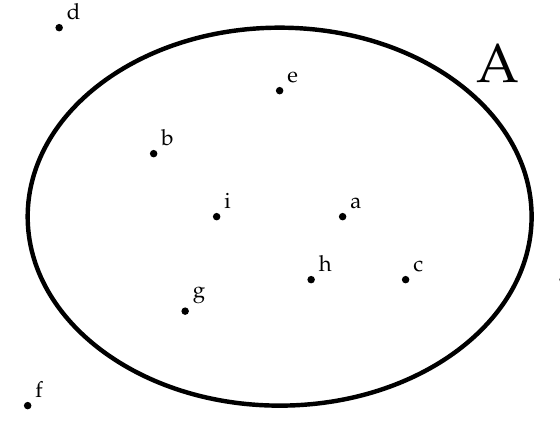
\begin{tikzpicture}[scale=.8,transform shape]
      \path[use as bounding box] (-4,-3) rectangle (4,3);
      \draw[ultra thick] (0,0) ellipse (4cm and 3cm);
      \node[anchor=south west] at (3,2) {\Huge A};
      \element{1,0}{a};
      \element{-2,1}{b};
      \element{2,-1}{c};
      \element{-1,0}{i};
      \element{0,2}{e};
      \element{0.5,-1}{h};
      \element{-1.5,-1.5}{g};

      \element{-4,-3}{f};
      \element{-3.5,3}{d};
      \element{4.5,-1}{j};
    \end{tikzpicture}
    \vskip5mm
     \[
      \begin{array}{c@{\qquad}c@{\qquad}c@{\qquad}c@{\qquad}c}
        \@a \in \@A & \@b \in \@A & \@c \in \@A & \@d \notin \@A & \@e \in \@A \\
        \@f \notin \@A & \@g \in \@A & \@h \in \@A & \@i \in \@A & \@j \notin \@A
      \end{array}
    \]
 \end{center}
\end{frame}
}

\begin{frame}
  \frametitle{Notaties}
  \begin{center}
    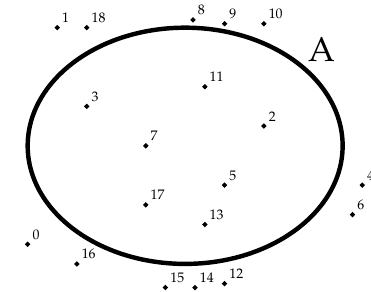
\begin{tikzpicture}[scale=.5,transform shape]
      \path[use as bounding box] (-4,-3) rectangle (4,3);
      \draw[ultra thick] (0,0) ellipse (4cm and 3cm);
      \node[anchor=south west] at (3,2) {\Huge A};
      \element{2,0.5}{2};
      \element{-2.5,1}{3};
      \element{1,-1}{5};
      \element{-1,0}{7};
      \element{0.5,1.5}{11};
      \element{0.5,-2}{13};
      \element{-1,-1.5}{17};

      \element{-4,-2.5}{0};
      \element{-3.25,3}{1};
      \element{4.5,-1}{4};
      \element{4.25,-1.75}{6};
      \element{.2,3.2}{8};
      \element{1,3.1}{9};
      \element{2,3.1}{10};
      \element{1,-3.5}{12};
      \element{.25,-3.6}{14};
      \element{-.5,-3.6}{15};
      \element{-2.75,-3}{16};
      \element{-2.5,3}{18};
    \end{tikzpicture}
  \end{center}
  \structure{Opsomming}
  \[ A = \left\{\; 2,3,5,7,11,13,17 \;\right\} \]
  \structure{Omschrijving}
  \[ A = \left\{\; x \;|\; x \leq 18 \textrm{ en } x \text{ is een priemgetal} \;\right\} \]
  \structure{Lege verzameling}
  \[ \emptyset = \{ \; \} \]
\end{frame}

\begin{frame}
  \frametitle{Gelijkheid}
  \begin{itemize}
    \item Twee verzamelingen $X$ en $Y$ zijn gelijk indien
          \[ \forall \; x. \; x \in X \iff x \in Y \]
          \vskip5mm
    \item In woorden
          \begin{center}
            $X$ en $Y$ zijn gelijk indien ze dezelfde elementen bevatten
          \end{center}
          \vskip5mm
    \item Notatie: $X = Y$
  \end{itemize}
\end{frame}

\begin{frame}
  \frametitle{Gevolgen}
  \begin{itemize}
    \item Een verzameling telt \emph{niet} hoe vaak een element voorkomt.
          \[ \{ 1, 1, 1, 1, 1 \} = \{ 1 \} \]
    \item Een verzameling definieert geen volgorde.
          \[ \{ 1, 2, 3 \} = \{ 3, 2, 1 \} \]
  \end{itemize}
\end{frame}

\begin{frame}
  \frametitle{Oefening 1.2}
  Gegeven de verzamelingen
  \[
    A = \left\{ 2,4,6,8,10 \right\}
    \qquad
    B = \left\{ 1,3,6,7,8 \right\}
  \]
  Welke uitspraken zijn waar?
  \[
    \begin{array}{l@{\hspace{2cm}}l}
      2 \in A & 11 \in B \\[2mm]
      4 \not\in B & \left\{2\right\} \in A \\[2mm]
      A \in \mathbb{N} & A = \left\{ \; x \;|\; x \in \mathbb{N} \textrm{ en $x$ is even} \right\}
    \end{array}
  \]
\end{frame}

\begin{frame}
  \frametitle{Deelverzameling}
  \begin{center}
    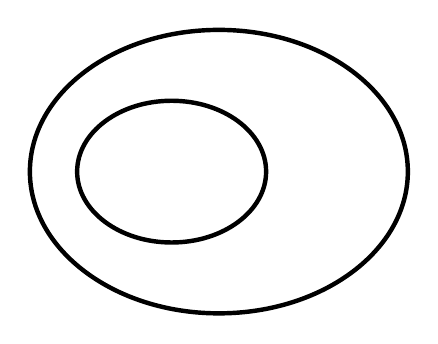
\begin{tikzpicture}[scale=.6,transform shape]
      \draw[ultra thick] (0,0) ellipse (4cm and 3cm);
      % \node[anchor=south west] at (3,2) {\Huge A};

      \draw[ultra thick] (-1,0) ellipse (2cm and 1.5cm);
      % \node[anchor=south west] at (.5,1) {\Huge B};
    \end{tikzpicture}
  \end{center}
  \begin{itemize}
    \item $X$ is een deelverzameling van $Y$ indien elk element van $X$ ook voorkomt in $Y$
          \[
            \forall \; x. \; x \in X \rightarrow x \in Y
          \]
    \item Notatie: $X \subset Y$
  \end{itemize}
\end{frame}

\begin{frame}
  \frametitle{Gevolgen}
  \begin{itemize}
    \item De lege verzameling is deelverzameling van elke verzameling
          \[ \emptyset \subset X \]
          \vskip4mm
    \item Link met gelijkheid
          \[ X \subset Y \quad\textrm{en}\quad Y \subset X \qquad\iff\qquad X = Y \]
  \end{itemize}
\end{frame}

\begin{frame}
  \frametitle{Unie}
  \begin{center}
    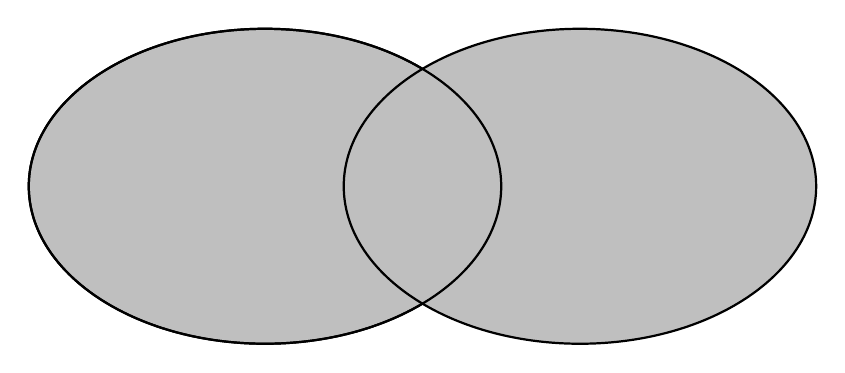
\begin{tikzpicture}
      \draw[highlight] \leftellipse;
      \draw[highlight] \rightellipse;
      \draw[outline] (-2,0) \leftellipse;
    \end{tikzpicture}
  \end{center}
  \[
    X \union Y = \{ \; x \;|\; x \in X \;\mathrm{of}\; x \in Y \; \}
  \]
\end{frame}

\begin{frame}
  \frametitle{Doorsnede}
  \begin{center}
    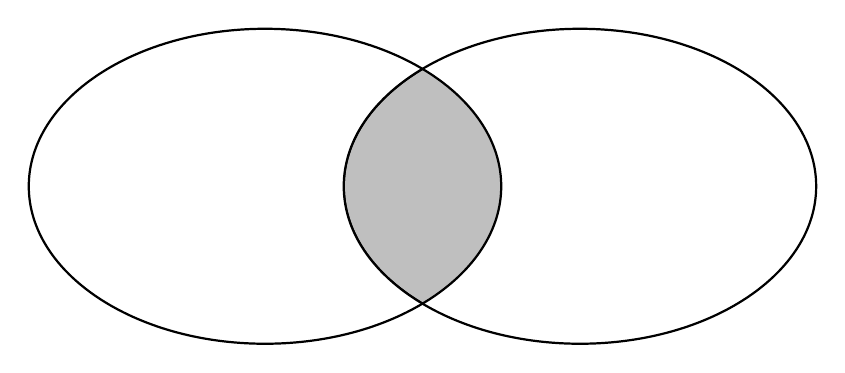
\begin{tikzpicture}
      \begin{scope}
        \clip \leftellipse;
        \clip \rightellipse;
        \draw[highlight] \leftellipse;
        \draw[highlight] \rightellipse;
      \end{scope}
      \draw[outline] \leftellipse;
      \draw[outline] \rightellipse;
    \end{tikzpicture}
  \end{center}
  \[
    X \intersect Y = \{ \; x \;|\; x \in X \;\mathrm{en}\; x \in Y \; \}
  \]
  \begin{itemize}
    \item $X$ is \emph{conjunct} met $Y$ als $X \intersect Y \neq \emptyset$
    \item $X$ is \emph{disjunct} met $Y$ als $X \intersect Y = \emptyset$
  \end{itemize}
\end{frame}

\begin{frame}
  \frametitle{Verschil}
  \begin{center}
    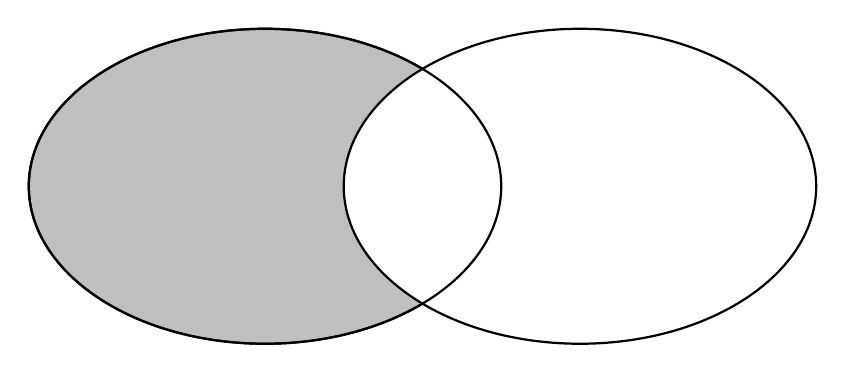
\begin{tikzpicture}
      \draw[highlight] \leftellipse;
      \draw[empty] \rightellipse;
      \draw[outline] \leftellipse;
    \end{tikzpicture}
  \end{center}
  \[
    X - Y = \{ \; x \;|\; x \in X \;\mathrm{en}\; x \notin Y \; \}
  \]
\end{frame}

\begin{frame}
  \frametitle{Complement}
  \begin{center}
    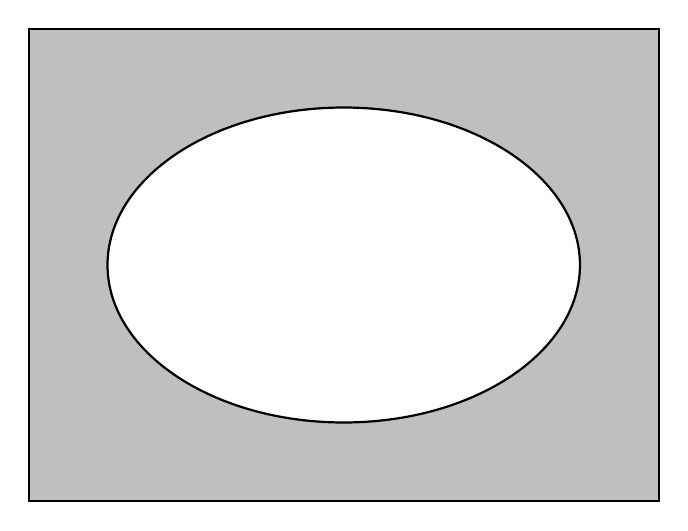
\begin{tikzpicture}
      \draw[highlight] (-4,-3) rectangle (4,3);
      \draw[empty] (0,0) ellipse (3cm and 2cm);
    \end{tikzpicture}
  \end{center}
  \[
    X^c = \{ \; x \;|\; x \in U \;\mathrm{en}\; x \notin X \; \} = U - X
  \]
\end{frame}

\begin{frame}
  \frametitle{Oefening}
  Vereenvoudig de volgende uitdrukkingen:
  \[
    \begin{array}{c}
      A \union A \\[2mm]
      A \intersect A \\[2mm]
      A - A \\[2mm]
      (A \union B) - B \\[2mm]
      (A \union B) \intersect A \\[2mm]
      (A^c)^c
    \end{array}
  \]
\end{frame}

\begin{frame}
  \frametitle{Cartesisch product}
  \begin{center}
    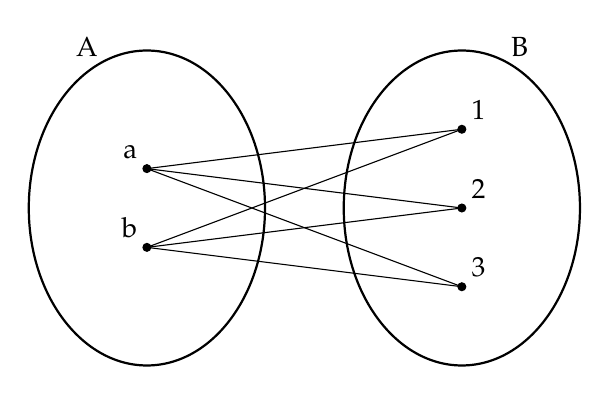
\begin{tikzpicture}
      \draw[outline] (-2,0) ellipse (1.5cm and 2cm);
      \node[anchor=south east] at (-2.5,1.8) {A};
      \draw[outline] (2,0) ellipse (1.5cm and 2cm);
      \node[anchor=south west] at (2.5,1.8) {B};

      \element[anchor=south east]{-2,0.5}{a}
      \element[anchor=south east]{-2,-0.5}{b}
      \element{2,1}{1}
      \element{2,0}{2}
      \element{2,-1}{3}

      \foreach \x in {0.5,-0.5} {
        \foreach \y in {1,0,-1} {
          \draw (-2,\x) -- (2,\y);
        }
      }
    \end{tikzpicture}
  \end{center}
  \[
    \begin{array}{rcl}
      \mathrm{A} & = & \left\{ \mathrm{a}, \mathrm{b} \right\} \\
      \mathrm{B} & = & \left\{ 1, 2, 3 \right\} \\
      \mathrm{A} \times \mathrm{B} & = & \left\{ ( \mathrm{a}, 1 ), (\mathrm{a}, 2 ), (\mathrm{a}, 3 ), ( \mathrm{b}, 1 ), (\mathrm{b}, 2 ), (\mathrm{b}, 3 ) \right\}
    \end{array}
  \]
  \vskip2mm
  \[
    X \times Y = \left\{ \; (x, y) \;|\; x \in X \;\mathrm{en}\; y \in Y \right\}
  \]
\end{frame}

\begin{frame}
  \frametitle{Rekenregels}
  \structure{Associativiteit}
  \[
    \begin{array}{rclclr}
      X \union (Y \union Z) & = & (X \union Y) \union Z & = & X \union Y \union Z \\
      X \intersect (Y \intersect Z) & = & (X \intersect Y) \intersect Z & = & X \intersect Y \intersect Z \\
    \end{array}
  \]
  \structure{Commutativiteit}
  \[
    \begin{array}{rcl}
      X \union Y & = & Y \union X \\
      X \intersect Y & = & Y \intersect X
    \end{array}
  \]
  \structure{Distributiviteit}
  \[
    \begin{array}{rcl}
      X \union (Y \intersect Z) & = & (X \intersect Y) \union (X \intersect Z) \\
      X \intersect (Y \union Z) & = & (X \union Y) \intersect (X \union Z) \\
    \end{array}
  \]
\end{frame}

\begin{frame}
  \frametitle{Rekenregels}
  \structure{Lege verzameling}
  \[
    \begin{array}{rclclr}
      X \union \emptyset & = & X \\
      X \intersect \emptyset & = & \emptyset \\
      X - \emptyset & = & X \\
      \emptyset - X & = & \emptyset \\
    \end{array}
  \]

  \structure{Wetten van de Morgan}
  \[
    \begin{array}{rclclr}
      (X \union Y)^c & = & X^c \intersect Y^c \\
      (X \intersect Y)^c & = & X^c \union Y^c \\
    \end{array}
  \]
\end{frame}

\begin{frame}
  \frametitle{Oefening 1.11}
  Geef door opsomming:
  \[
    \begin{array}{c}
      \left\{ \; x \in \mathbb{R} \;|\; (x-1) \cdot (x-2) = 6 \; \right\} \\[1cm]
      \left\{ \; 10\cdot x \;|\; x \in \mathbb{Z} \; \right\} \\[1cm]
      \left\{ \; 10 \in \mathbb{N} \;|\; x \textrm{ is een deler van 6} \; \right\} \\[1cm]
      \left\{ \; (x, y) \in A \times B \;|\; y = x - 10 \; \right\} \\ A = \{10,11,\dots,20\} \qquad B = \{0,1,\dots,6\}
    \end{array}
  \]
\end{frame}

\end{document}



%%% Local Variables: 
%%% mode: latex
%%% TeX-master: t
%%% End: 
